\documentclass{beamer}
\mode<presentation>
{
  \usetheme{default}      % or try Darmstadt, Madrid, Warsaw, ...
  \usecolortheme{default} % or try albatross, beaver, crane, ...
  \usefonttheme{default}  % or try serif, structurebold, ...
  \setbeamertemplate{navigation symbols}{}
  \setbeamertemplate{caption}[numbered]
} 

\usepackage[english]{babel}
\usepackage[utf8x]{inputenc}
\usepackage[numbers]{natbib}

\usepackage{geometry}

\usepackage{subcaption}
\usepackage{amsmath}
\usepackage{mathtools}
\DeclarePairedDelimiter\abs{\lvert}{\rvert}%
\DeclarePairedDelimiter\norm{\lVert}{\rVert}%

\title[Hacking the Xgboost]{Coupon Challenge}
\author{Raul Sanchez-Vazquez}
\institute{}
\date{25 June 2018}

\begin{document}

\begin{frame}
  \titlepage
  
\end{frame}

\begin{frame}{The Problem}
	
	The problem:
	
	\begin{itemize}
		\item 	Create a recommender system for coupons.
	\end{itemize}

	This would be done in two stages:
		\begin{itemize}
			\item 	First, learn a model for classic top-n recommendation.
			\item 	Second, learn a binary classification model where the positive class correspond to actual purchase of the item.
		\end{itemize}
		
	Produce recommendation as:
	\begin{itemize}
		\item 	Produce candidate items (RecSys Model)
		\item 	Order by purchase probability (Positive probability score)
	\end{itemize}
\end{frame}
	
\begin{frame}{Analysis}
	
	We first built data profiling documents for:
	
	\begin{itemize}
		\item The item catalog.
		\item The user catalog.
		\item The user session log with purchase information.
	\end{itemize}
	
	We first noticed that the binary classification model would have to deal with class unbalance as shown on the plot below: 
	
	\begin{figure}
		\centering
		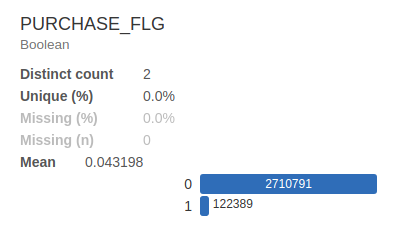
\includegraphics[width=0.7\linewidth]{../img/target}
		\caption{}
		\label{fig:target}
	\end{figure}
\end{frame}

\begin{frame}{Features}
	Item features:
	
\begin{itemize}
	\tiny
	\item itemd aged promo
	\item itemd nd views
	\item itemd nd purchases
	\item itemd area
	\item itemd ken
	\item itemd smalld area
	\item itemd kend mostd buy
	\item itemd kend mostd buy2
	\item itemd larged aread mostd buy
	\item itemd larged aread mostd buy2
	\item itemd smalld aread mostd buy
	\item itemd smalld aread mostd buy2
	\item itemd buyersd aged mean
	\item itemd buyersd aged median
	\item itemd buyersd aged std
	\item itemd DISCOUNTd PRICEd percentage
	\item itemd price
	\item itemd purchased sexd f
	\item itemd purchasesd sexd m
\end{itemize}
\end{frame}

\begin{frame}{Features}
	User features:
	\begin{itemize}
			\tiny
		\item userd samed itemd nd views
		\item userd samed itemd nd purchases
		\item userd lastd itemd larged aread name
		\item userd lastd itemd kend name
		\item userd lastd itemd smalld aread name
		\item userd purchasesd samed itemd area
		\item userd purchasesd samed itemd kend name
		\item userd purchasesd samed itemd smalld area
		\item userd AGE
		\item userd SEXd ID
	\end{itemize}
\end{frame}

\begin{frame}{Model Performace}

	Recsys on Test:
	\begin{itemize}
		\item P@10: 0.0018949648 
	\end{itemize}
	 
	Binary Classification on Test: 
		\begin{itemize}
			\item AUC:0.900254
		\end{itemize}
	
	\begin{figure}
	\centering
	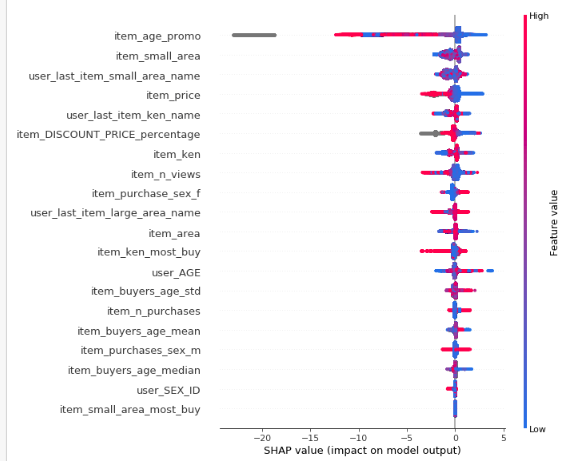
\includegraphics[width=0.7\linewidth]{../img/shap}
	\label{fig:shap}
	\end{figure}
\end{frame}

\begin{frame}{Model Performace}
	Hybrid recommender:

	\begin{itemize}
		\item P@10: 0.029458179905312992
	\end{itemize}
	
\end{frame}
	
\end{document}